\documentclass[11pt]{article}
\usepackage[UTF8]{ctex}
\usepackage[a4paper]{geometry}
\geometry{left=2.0cm,right=2.0cm,top=2.5cm,bottom=2.5cm}

\usepackage{comment}
\usepackage{booktabs}
\usepackage{graphicx}
\usepackage{diagbox}
\usepackage{amsmath,amsfonts,graphicx,amssymb,bm,amsthm}
\usepackage{algorithm,algorithmicx}
\usepackage[noend]{algpseudocode}
\usepackage{fancyhdr}
\usepackage{tikz}
\usepackage{graphicx}
\usepackage{verbatim}
\usetikzlibrary{arrows,automata}
\usepackage{hyperref}

\setlength{\headheight}{14pt}
\setlength{\parindent}{0 in}

\newtheorem{theorem}{Theorem}
\newtheorem{lemma}[theorem]{Lemma}
\newtheorem{proposition}[theorem]{Proposition}
\newtheorem{claim}[theorem]{Claim}
\newtheorem{corollary}[theorem]{Corollary}
\newtheorem{definition}[theorem]{Definition}


\newcommand\E{\mathbb{E}}
\newcommand{\hwid}{3}			% 第几次作业
\newcommand{\name}{周雨扬} 		% 你的名字
\newcommand{\id}{2000013061} 	% 你的学号


\usetikzlibrary{positioning}

\begin{document}

    \pagestyle{fancy}
    \lhead{Peking University}
    \chead{}
    \rhead{Operating Systems}

    \begin{center}
        {\LARGE \bf Homework \#\hwid}\\
        {\Large \name}\\
        {\Large \id}\\
    \end{center}

	\section{Challanges}
		\par 本次作业完成了所有的代码补全任务,做了如下的 Challange:
		\begin{itemize}
			\item Modify the JOS kernel monitor so that you can 'continue' execution from the current location (e.g., after the int3, if the kernel monitor was invoked via the breakpoint exception), and so that you can single-step one instruction at a time. You will need to understand certain bits of the EFLAGS register in order to implement single-stepping.
		\end{itemize}
		
	\section{Exercise 1}
	
		
	\subsection*{mem\_init()}
		\par 我们只需要声明用于存储页链表 \texttt{envs} 的内存即可。因此可以通过直接调用 \texttt{boot\_alloc} 解决。代码可以见 \texttt{kern/pmap.c, Line 177 $\sim$ 179 ,210}。
		
	\subsection*{备注}
		由于不明原因,我修改了初始化时侯的部分内存分配,增加了 \texttt{kern/pmap.c, Line 149}。如果不直接添加。其会导致存储 \texttt{kern\_pgdir} 的地址,恰好落在 \texttt{[kern\_pgdir, kern\_pgdir + PGSIZE)} 区间内,这意味着随着两行后的 \texttt{memset} 指令,就会将指针 \texttt{kern\_pgdir} 指向的地址赋为 0.
		
		产生的原因不是 Lab1 的代码因为 Lab1 几乎没有改动,错误产生的位置在 Lab2 所有改动之前,因此我怀疑是链接器/链接文件出了些bug。
		
	\section{Exercise 2}
	
	\subsection*{env\_init()}
	
		我们需要将所有的空环境用链表的形式进行存储,且使得最后的 \texttt{env\_free\_list} 指向 \texttt{envs[0]}。因此我们直接按描述建立即可。代码可以见 \texttt{kern/env.c, Line 120 $\sim$ 125}。
		
		注意由于我们分配的时候已经赋值为 0,因此不需要设置初始 id 为 0.
		
	
	\subsection*{env\_setup\_vm()}
	
		我们可以利用已经创建好的页表 \texttt{kern\_pgdir} 作为模板拷贝到新的环境页表中。之后直接将新页表下标赋值给环境即可。代码可以见  \texttt{kern/env.c, Line 189 $\sim$ 191}。
		
		注意由于我们需要手动增加新页表的引用数。
	
	\subsection*{region\_alloc()}
	
		首先我们需要将映射的内存按照整页进行上下取整(因为我们采用整页管理)。之后,我们可以直接依序利用 Lab2 中的页声明函数 \texttt{page\_alloc()} 和页插入函数 \texttt{page\_insert} 将页插入到当前环境的虚拟内存中即可。代码可以见  \texttt{kern/env.c, Line 280 $\sim$ 288}。
		
		
	\subsection*{load\_icode()}
	
		首先我们需要检查 \texttt{ELF} 头中的 \texttt{e\_magic} 项是否正确。如果不正确则无法执行需要退出;否则我们首先需要切换页表。观察发现下面的代码我们可以使用 \texttt{lcr3()} 来实现该操作。
		
		之后我们就可以利用 \texttt{ELF} 头求出程序描述符 \texttt{Proghdr}, 并求出代码中每一段的信息。由于我们只需要将属性为 \texttt{ELF\_PROG\_LOAD} 的每一段进行插入,我们可以直接使用 \texttt{region\_alloc()} 分配内存后简单的 \texttt{memcpy} 即可。多余的部分将其赋值为 $0$。
		
		最后我们需要将页表切换回内核态的页表,同时设置插入点。观察发现点为 \texttt{env\_tf.tf\_eip},就可以完成代码。代码可以见  \texttt{kern/env.c, Line 346 $\sim$ 361}。
		
	\subsection*{env\_create()}
		根据 lab 上面的提示编写即可。注意我们已经在声明存储环境的空间是,将 \texttt{parent ID} 设置为 0 了。代码可以见  \texttt{kern/env.c, Line 381 $\sim$ 386}。
	
	\subsection*{env\_run()}
		如果当前存在运行进程,则我们首先需要将其切出,之后再将当前环境设置为 \texttt{ENV\_RUNNING}。注意之后的所有寻址都是在当前环境的页表下进行,因此需要切换页表根节点。
		
		之后根据描述我们只需要调用 \texttt{env\_pop\_tf} 并传入对应参数即可。代码可以见  \texttt{kern/env.c, Line 503 $\sim$ 513}。
		
	\section{Exercise 4}
		
		\subsection*{trapentry.S}
		
			观察代码,发现其引用了 \texttt{inc/trap.h},其中共有 $20$ 种中断与异常类型。查阅相关材料可以直接确定每一种异常/中断是否需要在栈中压入 \texttt{error code}. 据此我们可以首先在文件中声明每一种错误的入口函数。代码可以见  \texttt{kern/trapentry.S, Line 50 $\sim$ 70}。
			
			
			之后我们需要完善 \texttt{\_alltraps}。观察 \texttt{Trapframe} 和文档我们发现系统已经帮我们实现压入了 \texttt{trap\_no} 之后的部分,\texttt{trap\_no}在声明异常函数的时候已经被压入,此时我们只需要压入 \texttt{\%ds,\%es} 和所有的寄存器即可。之后的指令可以直接按照文档里给出的写。代码可以见 \texttt{kern/trapentry.S, Line 76 $\sim$ 87}。
	
		\subsection*{trap\_init()}
			 此时我们需要声明 \texttt{idt} 数组。我们发现所有的中断都会重设 \texttt{IF} 位,因此 \texttt{istrap = 0}; \texttt{kernel code segment} 在 \texttt{kern/env.h} 出现过,因此其值位 \texttt{GD\_KT};最后两项依次位函数入口和权限级别。函数接口我们在 \texttt{trapentry} 已经声明过,其类型为 \texttt{void()};权限目前可以统一设置为内核级(0)。
			 
			 据此我们完成了其初始化,代码可以见 \texttt{kern/trap.c, line 66 $\sim$ 106}。
		
		\subsection*{question 1}
			如果所有异常都使用同一个 handler,一会出现安全问题,因为不同异常操作权限不同;二也不利于多个异常同时抛出情况下内核的处理。
	
		\subsection*{question 2}
			因为页错误的权限位是 0,我们不希望用户能够抛出页错误。
			
			如果我们将权限位设为 3(用户态),则用户就可以抛出该错误,但这不是我们所希望的:用户不能也不应该干涉内存管理。
	
	\section{Exercise 5,6}
	
		\subsection*{trap\_dispatch()}
			观察到页错误和端点分别对应了 \texttt{T\_PGFLT} 和 \texttt{T\_BRPKT}, 对应需要执行的函数是 \texttt{page\_fault\_handler()} 和 \texttt{moniter}, 因此直接实现即可。但是这样断点会错误,因为其是在用户态下被发送的,我们需要额外在 \texttt{idt} 种修改其权限位为 3。代码可以见 \texttt{kern/trap.c, line 186 $\sim$ 192}。
		
		\subsection*{question 3}
			类似于 \texttt{question 2},如果我们设置只有系统能够产生该中断,则会产生\texttt{general protection fault},因为用户权限不足。
			
			为此我们才需要额外在 \texttt{idt} 种修改其权限位为 3。这样用户才能产生端点错误,系统便能够正确捕捉了。
			
		\subsection*{question 4}
			为了保护系统,不让用户干涉某些重要过程。
	
	\section{Exercise 7}
	
		\subsection*{trap\_dispatch()}
			由于用户可以发起系统调用,因此我们需要将其权限位设置为 $3$。查阅资料发现系统调用的参数依次为 \texttt{\%edx, \%ecx, \%ebx, \%edi, \%esi},因此我们直接调用 \texttt{syscall} 函数并将其返回值存储在 \texttt{\%eax} 中即可。该部分代码可以见 \texttt{kern/trap.c, line 193 $\sim$ 200}
		
		\subsection*{syscall()}
		根据描述我们只需要利用一个 \texttt{switch} 语句判断其执行的命令即可。注意参数是按照 \texttt{a1,a2} 的顺序传输,在命令错误时只需要返回 \texttt{-E\_INVAL}.该部分代码可以见 \texttt{kern/syscall.c, line 75 $\sim$ 87}
		
	\section{Exercise 8}
		
		\subsection*{libmain()} 
		由于我们已经声明了存储环境信息的内存 \texttt{envs},因此我们只需要获取环境编号即可。获取编号可以使用 \texttt{sys\_getenvid},利用编号获取偏移可以使用 \texttt{ENVX},简单实现即可。该部分代码可以见 \texttt{lib/libmain.c, line 16}.
		
	\section{Exercise 9}
	
	\subsection*{page\_fault\_handler()} 
		观察代码发现, \texttt{tf\_cs} 的最低两位恰好代表环境的权限位。基于此可以简单地实现,代码可以见\texttt{lib/libmain.c, line 265 $\sim$ 266}.
		
	\subsection*{user\_mem\_assert()} 
		类似于 \texttt{region\_alloc()},我们可以首先获取需要检查的页,对于每一个页,我们利用 \texttt{pgdir\_walk()} 获取该页的信息,并检查该页的信息是否存在,是否越界,权限是否合法。注意最后生成的 \texttt{user\_mem\_check\_addr} 需要和 \texttt{va} 取较大者。代码可以见\texttt{kern/pmap.c, line 577 $\sim$ 586}.
		
	\subsection*{sys\_cputs()}
		利用 \texttt{user\_mem\_assert} 检查对应内存区间权限即可。代码可以见\texttt{kern/syscall.c, line 24}.
		
	\subsection*{debug\_eip\_info()}
	类似的利用 \texttt{user\_mem\_check} 检查对应内存区间权限即可。代码可以见\texttt{kern/kdebug.c, line 145,154,155}.
	
	\subsection*{Challange 2}
		
		再出现 \texttt{int \$3} 之后我们会进入内核态,不再进行当前进程。但是我们实际上可以利用陷入时候的 \texttt{struct Trapframe *tf} 恢复原先状态。当然在恢复之前,我们需要检查传入的参数 \texttt{tf},判定其是否属于可以继续执行的状态。
		
		复原状态的时候,我们直接修改当前状态的 \texttt{env\_tf} 值为传入值即可。针对单步执行和继续执行两种不同的情况,查阅资料发现 \texttt{env\_tf} 中 \texttt{tf\_eflags} 的第 9 位(\texttt{0x100}) 恰好可以控制该性质,其值位 $1$ 的时候会进入单步状态。据此我们针对不同的任务对应修改即可。
		
		代码可以见\texttt{kern/moniter.c, line 182 $\sim$ 216}.
		
		运行结果如下图所示:
		
		
\begin{figure}
\centering
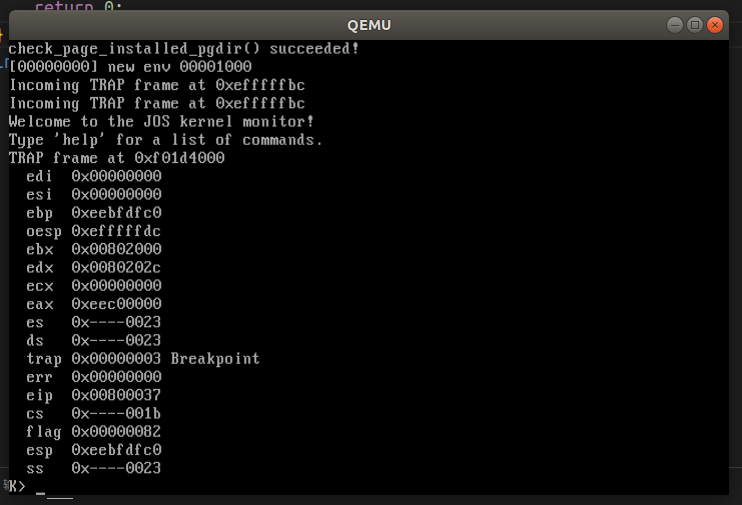
\includegraphics[width=0.7\linewidth]{kern.png}
\caption{运行 \texttt{make run\_breakpoint} 的结果}
\label{fig:kern}
\end{figure}

	
	\begin{figure}
		\centering
		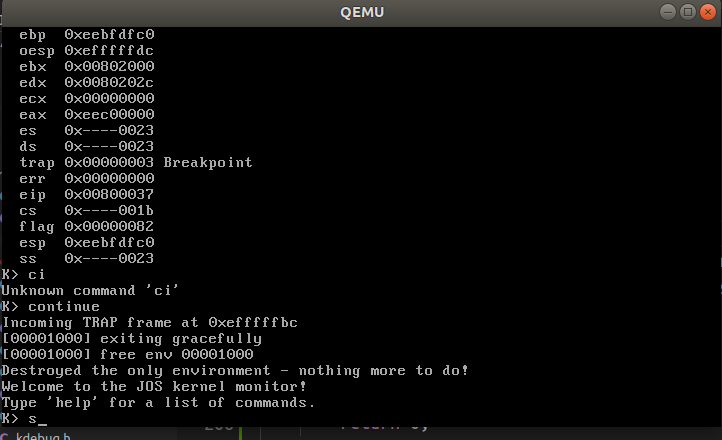
\includegraphics[width=0.7\linewidth]{cicici.png}
		\caption{运行 \texttt{ci/continue} 的结果}
		\label{fig:kern}
	\end{figure}
		 
			\begin{figure}
				\centering
				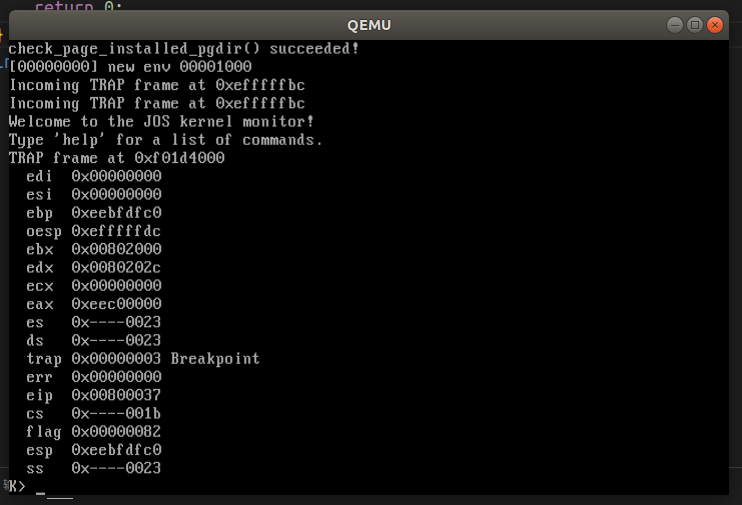
\includegraphics[width=0.7\linewidth]{si.png}
				\caption{运行 \texttt{s/si} 的结果}
				\label{fig:kern}
			\end{figure}
			
		
		
	
\end{document}